\documentclass[main.tex]{subfiles}

\begin{document}

\subsection{Terzo esercizio}

\begin{figure}[H]
\centering
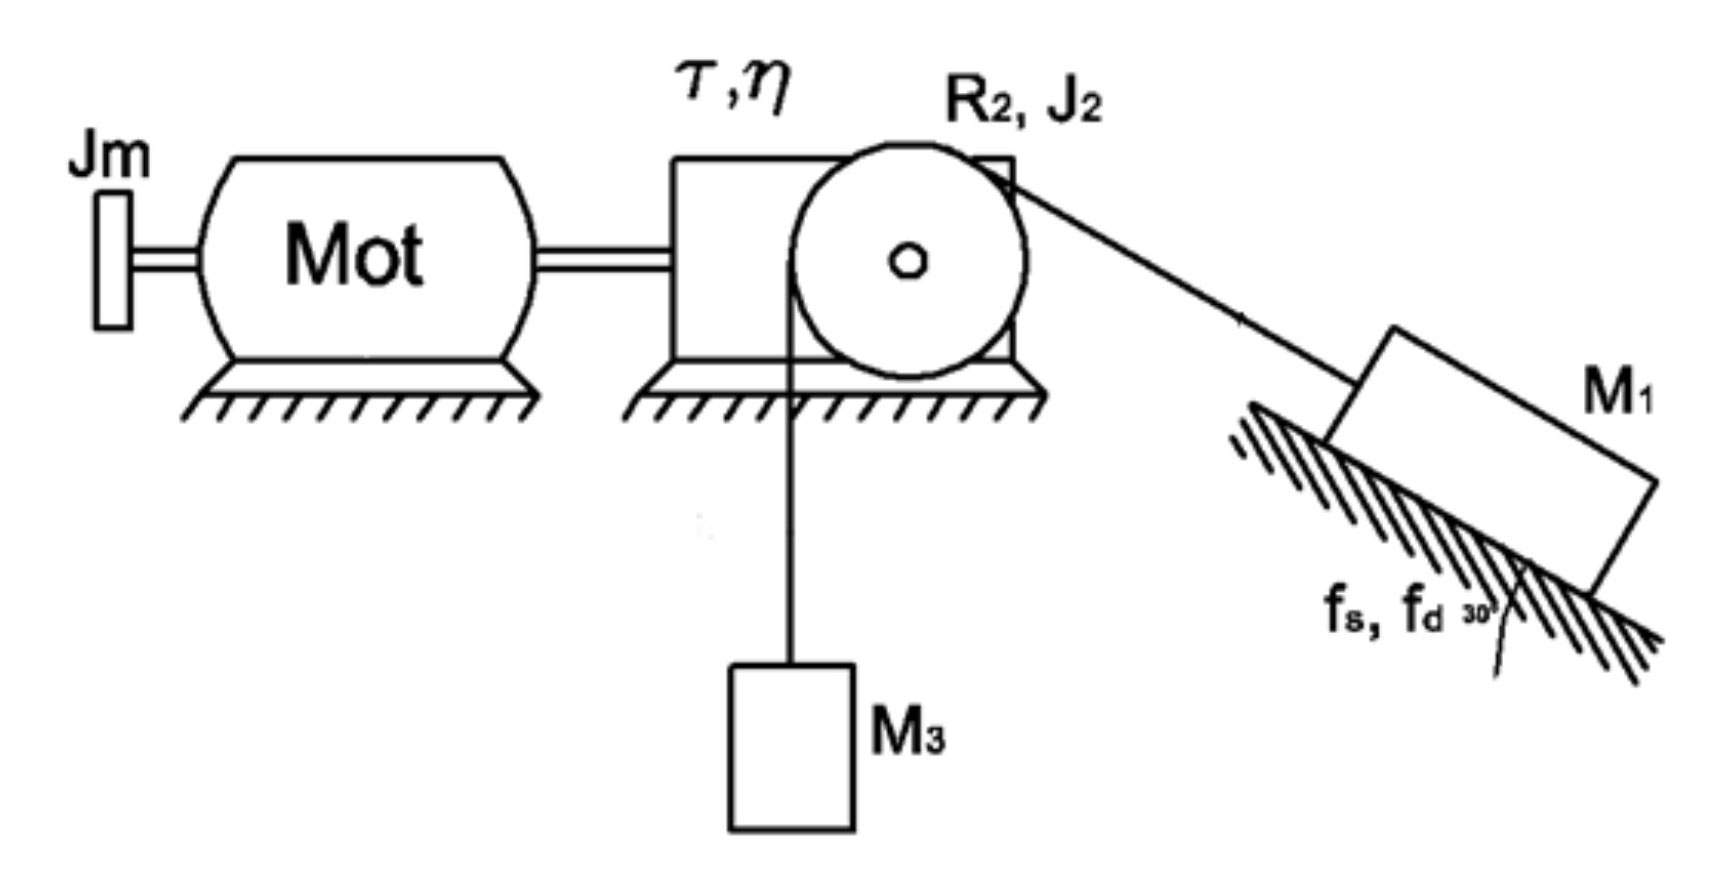
\includegraphics[width=0.75\textwidth]{2014-0407-3.jpg}
\end{figure}

\begin{figure}[H]
\centering
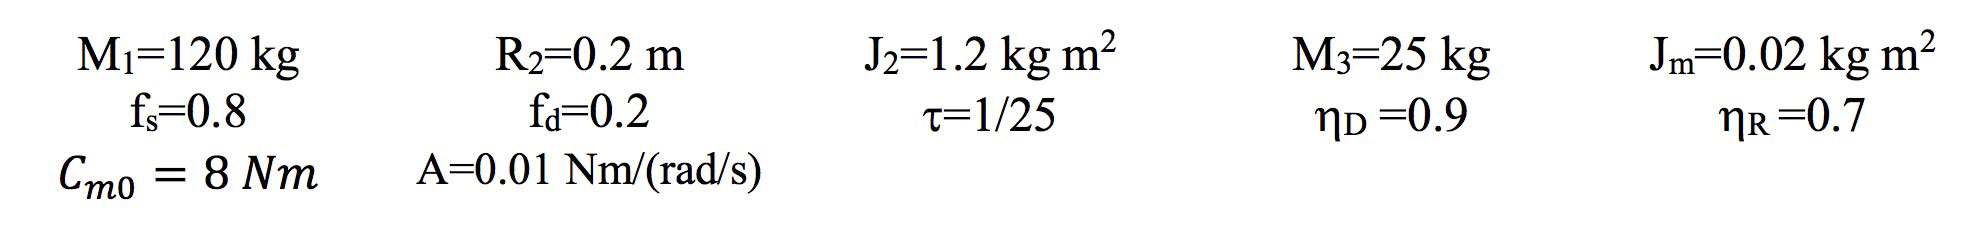
\includegraphics[width=\textwidth]{2014-0407-3-dati.jpg}
\end{figure}

L’impianto di sollevamento in figura è posto nel piano verticale ed è azionato attraverso un gruppo motore-riduttore di caratteristiche note: rapporto di riduzione $\tau$ e rendimento $\mu_D$ (per condizione di moto diretto) e $\mu_R$ (per condizione di moto retrogrado). È inoltre assegnata l’equazione che definisce la curva caratteristica del motore: $C_m = C_{m_0} - A\omega_m$.

Una fune inestensibile di massa trascurabile si avvolge su una puleggia di raggio $R_2$: a un’estremità della fune è collegata la massa la massa $M_1$ che si muove su un piano inclinato ($30\deg$), scabro (coefficiente di attrito statico e dinamico assegnati). All’altro estremo della fune è appeso il contrappeso $M_3$.

Si chiede di calcolare:
\begin{enumerate}
\item La coppia che deve fornire il motore nel caso di salita della massa $M_1$ lungo il piano inclinato a velocità costante.
\item La velocità della massa $M_1$ per la condizione di funzionamento di cui al punto 1.
\item La coppia motrice che deve fornire il motore affinchè la massa $M_1$ si muova in discesa, rallentando con una decelerazione pari a 0.5 m/s2.
\end{enumerate}

\clearpage

\subsection{Soluzione terzo esercizio}

\subsubsection{Osservazioni}

\begin{enumerate}
\item La velocità \textit{costante} implica che al primo primo ci si trova in condizioni di regime.
\item La massa M1 è sempre in moto, per cui va sempre usato il coefficiente di attrito dinamico $f_d$.
\item Nel terzo punto viene fornita una \textbf{decelerazione}, per cui andrà inserita come negativa.
\end{enumerate}

\subsubsection{Primo punto}

\paragraph{Identifico il legame cinematico} La velocità con cui i baricentri di $M_1$, $M_3$ ed un punto sulla circonferenza della puleggia è pari a $v = R_2\tau\omega_m$.

\paragraph{Potenza motrice}

\[
	W_m = C_m\omega_m
\]

\paragraph{Potenza resistente} Per calcolare la potenza resistente prendo in considerazione tutti gli oggetti in moto su cui venga applicata una forza, quindi $M_1$ con la forza peso e la forza d'attrito dinamico ed $M_3$ con la sola forza peso.

\[
	W_r = \vec{F}_{g_{M_3}}\bullet\vec{v}_3 + \vec{F}_{g_{M_1}}\bullet\vec{v}_1 + \vec{F}_{d_{M_3}}\bullet\vec{v}_1
\]

\begin{enumerate}
\item La forza peso agente su $M_3$ è concorde con la direzione della velocità $v_3$, cioè forma un angolo di $0\deg$.
\item La forza peso agente su $M_1$ forma un angolo di $\dfrac{\pi}{2} + \dfrac{\pi}{6}$ con la velocità $v_1$.
\item La forza di attrito dinamico agente su $M_1$ agisce in direzione opposta a $v_1$, cioè forma un angolo di $\pi$. La forza d'attrito dinamico è definita come: $\vec{F}_{d_{M_3}} = M_1gf_d\sin(\dfrac{\pi}{2}+\dfrac{\pi}{6})$
\end{enumerate}

Risolvo il prodotto \textbf{scalare}:

\begin{align*}
	W_r &= F_{g_{M_3}}v_3 + F_{g_{M_1}}v_1\cos\left( \dfrac{\pi}{2} + \dfrac{\pi}{6} \right ) - F_{d_{M_1}}v_1\\
	&= M_3gv - \dfrac{1}{2}M_1gv - M_1g f_d \cos(\dfrac{\pi}{6})v\\
	&= vg(M_3 - \dfrac{1}{2}M_1 - M_1 f_d \cos(\dfrac{\pi}{6}))\\
	&= vg(M_3 - M_1(\dfrac{1}{2} + f_d \cos(\dfrac{\pi}{6})))\\
	&= vg(M_3 - M_1(\dfrac{1}{2} + f_d\dfrac{\sqrt{3}}{2}))\\
\end{align*}

\paragraph{Identifico il tipo del moto} Siccome siamo in condizioni di regime, non è necessario calcolare la variazione di energia cinetica. Utilizzo la disequazione della potenza resistente per identificare il tipo di moto:

\[
	W_r > 0
\]

Se essa risulta vera, il moto è \textbf{retrogrado}, altrimenti \textbf{diretto}.

\[
	 vg(M_3 - M_1(\dfrac{1}{2} + f_d\dfrac{\sqrt{3}}{2}))>0
\]

\[
	-75.9vg>0
\]

L'equazione risulta falsa, per cui il moto è \textbf{diretto}.

\paragraph{Potenza perduta} Essendo in condizioni di regime e di moto diretto, uso la formula della potenza perdura seguente:

\[
	W_p = -(1-\mu_D)W_m
\]

\paragraph{Bilancio di potenze}

\[
	W_m + W_r + W_p = 0
\]

\[
	W_m + W_r -(1-\mu_D)W_m = 0
\]

\[
	W_r +\mu_DW_m = 0
\]

\[
	vg(M_3 - M_1(\dfrac{1}{2} + f_d\dfrac{\sqrt{3}}{2})) +\mu_DC_m\omega_m = 0
\]

\[
	\tau R_2\omega_m g(M_3 - M_1(\dfrac{1}{2} + f_d\dfrac{\sqrt{3}}{2})) +\mu_DC_m\omega_m = 0
\]

\[
	\tau R_2 g(M_3 - M_1(\dfrac{1}{2} + f_d\dfrac{\sqrt{3}}{2})) +\mu_DC_m = 0
\]

\[
	C_m = -\dfrac{\tau R_2 g(M_3 - M_1(\dfrac{1}{2} + f_d\dfrac{\sqrt{3}}{2}))}{\mu_D}
\]

\[
	C_m = 4.86\,Nm
\]

\subsubsection{Secondo punto}

\paragraph{Curva caratteristica del motore} Utilizzando l'equazione fornita, calcolo la velocità angolare del motore alla coppia calcolata al punto precedente. Quindi, sostituisco il valore ottenuto nel legame cinematico della velocità.

\[
	\omega_m = \dfrac{C_{m_0} -C_m}{A} = 313\,m/s
\]

\[
	v = R_2 \tau \omega_m = 2.5\,m/s
\]

\subsubsection{Terzo punto}

Ora, avendo una decelerazione non siamo più in condizioni di regime ma di transitorio. È quindi necessario calcolare la variazione di energia cinetica.

Inoltre la direzione della velocità è invertita, quindi sarà necessario invertire i segni del prodotto scalare della potenza resistente.

Sarà infine necessarrio re-identifare il tipo di moto in cui si trova il sistema.

\paragraph{Legame cinematico della decelerazione} Per utilizzare il dato della decelerazione vado a identificare un legame cinematico tra essa e l'accelerazione angolare.

$a = -R_2 \tau \dot{\omega}_m$

\paragraph{Energia cinetica}

\[
	E_c = \dfrac{1}{2}M_3v^2 + \dfrac{1}{2}M_1v^2 + \dfrac{1}{2}J_2(\tau\omega_m)^2 + \dfrac{1}{2}J_m\omega_m^2
\]

\[
	E_c = \dfrac{1}{2}M_3(R_2 \tau \omega_m)^2 + \dfrac{1}{2}M_1(R_2 \tau \omega_m)^2 + \dfrac{1}{2}J_2(\tau\omega_m)^2 + \dfrac{1}{2}J_m\omega_m^2
\]

\[
	E_c = \omega_m^2(\dfrac{1}{2}M_3(R_2 \tau)^2 + \dfrac{1}{2}M_1(R_2 \tau)^2 + \dfrac{1}{2}J_2(\tau)^2 + \dfrac{1}{2}J_m)
\]

Derivo l'espressione ed ottengo:
\[
	\dfrac{dE_c}{dt} = \omega_m\dot{\omega}_m((M_3+M_1)(R_2 \tau)^2 + J_2(\tau)^2 + J_m)
\]

\paragraph{Potenza resistente}

\begin{enumerate}
\item La forza peso agente sulla massa $M_3$ ora agisce in direzione opposta alla velocità di discesa.
\item La forza peso agente sulla massa $M_1$ forma un angolo di $\pi/3$ con la velocità.
\item La forza di attrito dinamico agisce sempre in direzione opposta alla velocità.
\end{enumerate}

\begin{align*}
	W_r &= -F_{g_{M_3}}v_3 + F_{g_{M_1}}v_1\cos\left(\dfrac{\pi}{6} \right ) - F_{d_{M_3}}v_1\\
	&= -M_3gv + M_1 g v\cos\left(\dfrac{\pi}{3} \right ) - M_1g f_d \cos(\dfrac{\pi}{6})v\\
	&= gv(-M_3 + M_1 \cos\left(\dfrac{\pi}{3} \right ) - M_1 f_d \cos(\dfrac{\pi}{6}))\\
	&= gv(M_1(\cos\left(\dfrac{\pi}{3} \right ) -  f_d \cos(\dfrac{\pi}{6}))-M_3)\\
\end{align*}

\paragraph{Identifico il tipo di moto}

\[
	W_r - \dfrac{dE_{c_r}}{dt} > 0
\]

\[
	gR_2 \tau(M_1(\cos\left(\dfrac{\pi}{3} \right ) -  f_d \cos(\dfrac{\pi}{6}))-M_3) - \dot{\omega}_m((M_3+M_1)(R_2 \tau)^2 + J_2(\tau)^2 + J_m) > 0
\]

Per la condizione di decelerazione, $\dot{\omega}_m = -\dfrac{a}{R_2 \tau} = -62.5\,rad/s^2$.

Tutti i termini della disequazione risultano quindi positivi e il moto è da considerarsi \textbf{retrogrado}.

\paragraph{Potenza perduta} Siamo in condizioni di transitorio e moto retrogrado. La formula da usare è quindi:

\[
	W_p = -(1-\mu_r)(W_r  - \dfrac{dE_{c_r}}{dt})
\]

\paragraph{Bilancio di potenze}

\[
	W_m + W_r + W_p = \dfrac{dE_{c_r}}{dt} + \dfrac{dE_{c_m}}{dt}
\]

\[
	W_m + W_r - (1-\mu_r)(W_r  - \dfrac{dE_{c_r}}{dt}) = \dfrac{dE_{c_r}}{dt} + \dfrac{dE_{c_m}}{dt}
\]

\[
	W_m  + \mu_r(W_r  - \dfrac{dE_{c_r}}{dt}) = \dfrac{dE_{c_m}}{dt}
\]

\[
	W_m  + \mu_r W_r  = \dfrac{dE_{c_m}}{dt} + \mu_r \dfrac{dE_{c_r}}{dt}
\]

\[
	C_m \omega_m  + \mu_r W_r  = \dfrac{dE_{c_m}}{dt} + \mu_r \dfrac{dE_{c_r}}{dt}
\]

\[
	C_m  = \dfrac{\dfrac{dE_{c_m}}{dt} + \mu_r \dfrac{dE_{c_r}}{dt} - \mu_r W_r}{\omega_m}
\]

\[
	C_m  = \dfrac{\omega_m\dot{\omega}_m(\mu_rM_3(R_2 \tau)^2 + \mu_rM_1(R_2 \tau)^2 + \mu_rJ_2(\tau)^2 +  J_m) -\mu_rgv(M_1(\cos\left(\dfrac{\pi}{3} \right ) -  f_d \cos(\dfrac{\pi}{6}))-M_3)}{\omega_m}
\]

\[
	C_m  = \dot{\omega}_m(\mu_r\tau^2((M_3+M_1)R_2^2 + J_2) + J_m) - \mu_rgR_2\tau(M_1(\cos\left(\dfrac{\pi}{3} \right ) -  f_d \cos(\dfrac{\pi}{6}))-M_3)
\]

\end{document}